%% Supplemental Material — EPD Model Movies
%% Compile separately: xelatex supplement.tex
\documentclass[aps,pre,twocolumn,floatfix]{revtex4-2}

\usepackage{amsmath,amssymb}
\usepackage{graphicx}
\usepackage{hyperref}
\usepackage{microtype}

\newcommand{\numes}{\nu_{\mathrm{meas}}}
\newcommand{\dA}{\Delta A}

\begin{document}

\title{Supplemental Material:\\
       Movies for ``The Elastic Perimeter Disk Model''}
\author{Research Note}
\date{\today}

\maketitle

This supplemental material provides six movies of two-disk squeeze simulations
at fixed $b = 0.2$, $N = 32$, $\varepsilon_\mathrm{ref} = 0.08$, illustrating
the squishiness axis as $q$ is varied from area-compressible to nearly
incompressible.  In all movies: the two EPD disks (blue/orange perimeter nodes)
are squeezed between rigid horizontal walls (gray); the color of each node
encodes the local contact force magnitude; the title shows current per-particle
strain $\varepsilon_p$ and instantaneous $\numes$.

All movies are provided as animated GIFs in the \texttt{movies/} subdirectory.

%%------------------------------------------------------------------
\section*{Movie S1 — Full squishiness sweep (comparison)}
%%------------------------------------------------------------------

\begin{figure}[htb]
  \centering
  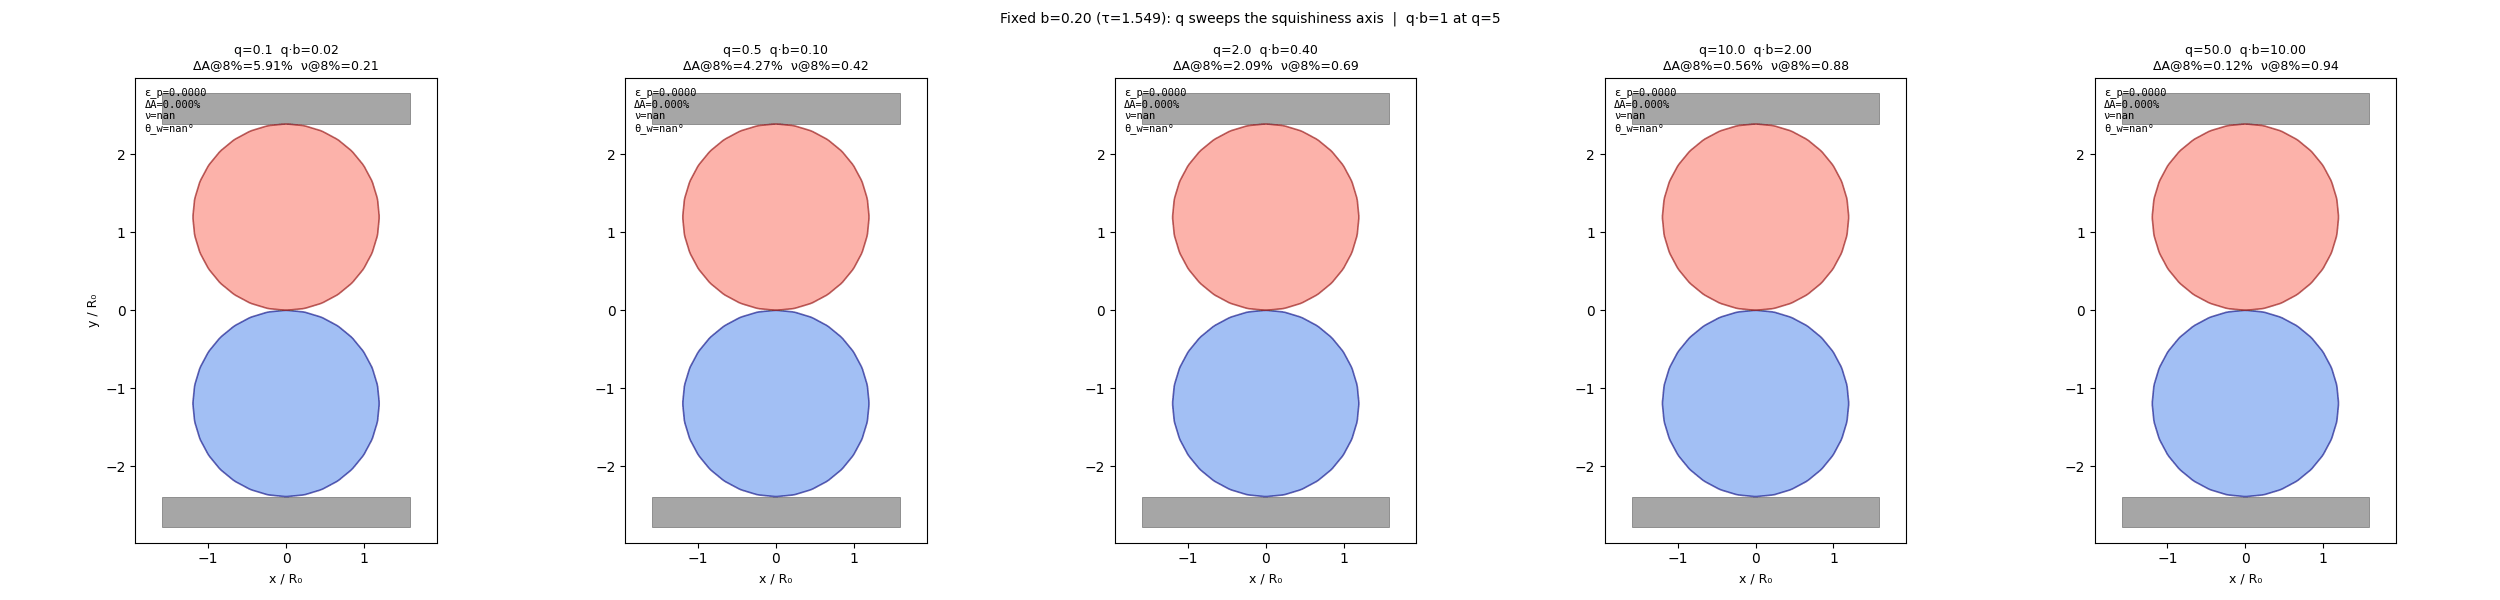
\includegraphics[width=\linewidth]{figures/S1_frame.png}
  \caption{%
    \textbf{Movie~S1} (\texttt{movies/S1\_comparison\_q\_sweep.gif}):
    Side-by-side comparison of five $q$ values
    ($q \in \{0.1, 0.5, 2, 10, 50\}$, left to right) at fixed $b = 0.2$, all
    compressed to the same wall displacement.  The visual transition from
    strongly flattened area-compressible shapes (left) to laterally bulging
    nearly-incompressible shapes (right) illustrates the full squishiness axis.
    Still shown: initial configuration ($\varepsilon_p = 0$).
  }
  \label{fig:S1}
\end{figure}

%%------------------------------------------------------------------
\section*{Movie S2 — Area-compressible disk ($q = 0.1$, $\numes \approx 0.21$)}
%%------------------------------------------------------------------

\begin{figure}[htb]
  \centering
  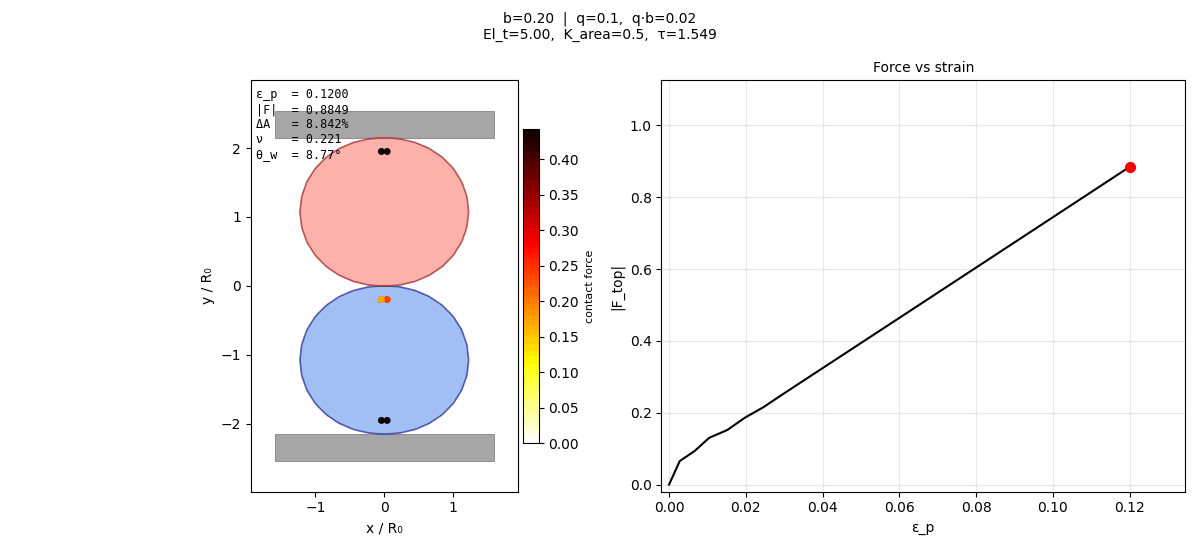
\includegraphics[width=\linewidth]{figures/S2_frame.png}
  \caption{%
    \textbf{Movie~S2} (\texttt{movies/S2\_q0p1\_area\_compressible.gif}):
    Single squeeze simulation at $q = 0.1$ ($q \cdot b = 0.02$,
    $\numes \approx 0.21$, $\dA \approx 5.9\%$).
    The area penalty is weak; the disk compresses largely in place with
    little lateral expansion.  The flattened top and bottom contact zones
    are clearly visible; the sides remain nearly straight.
    Still shown: maximum compression ($\varepsilon_p \approx 0.14$).
  }
  \label{fig:S2}
\end{figure}

%%------------------------------------------------------------------
\section*{Movie S3 — Compressible disk ($q = 0.5$, $\numes \approx 0.42$)}
%%------------------------------------------------------------------

\begin{figure}[htb]
  \centering
  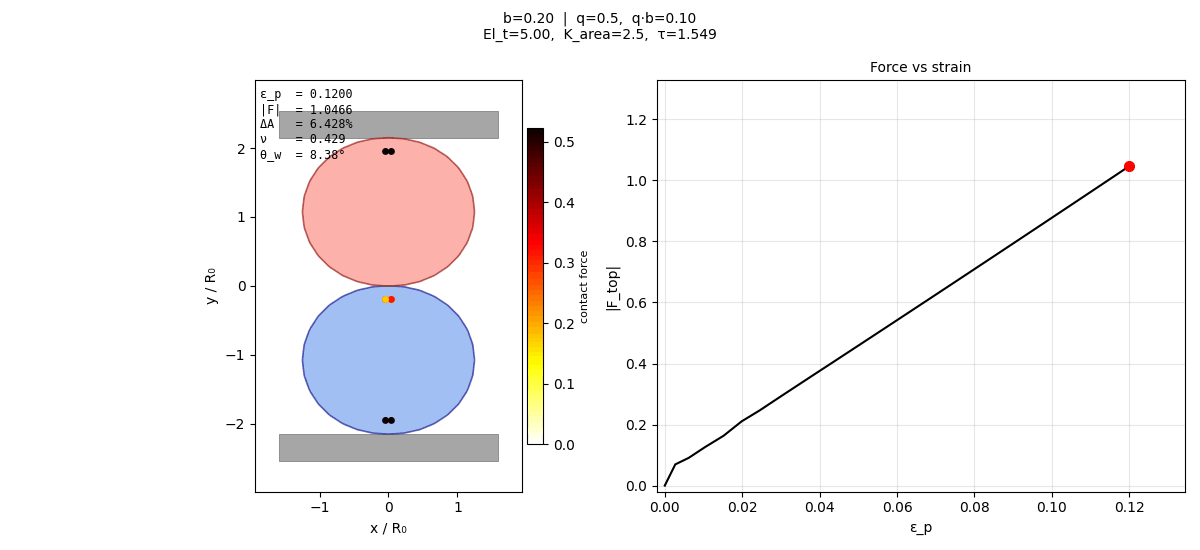
\includegraphics[width=\linewidth]{figures/S3_frame.png}
  \caption{%
    \textbf{Movie~S3} (\texttt{movies/S3\_q0p5\_compressible.gif}):
    Single squeeze at $q = 0.5$ ($q \cdot b = 0.10$, $\numes \approx 0.42$,
    $\dA \approx 4.3\%$).  Moderate area loss; the disk begins to bulge
    laterally.  The transition from predominantly area-compressible to
    mixed behavior is visible in the rounding of the equatorial cross-section.
    Still shown: maximum compression.
  }
  \label{fig:S3}
\end{figure}

%%------------------------------------------------------------------
\section*{Movie S4 — Intermediate disk ($q = 2.0$, $\numes \approx 0.69$)}
%%------------------------------------------------------------------

\begin{figure}[htb]
  \centering
  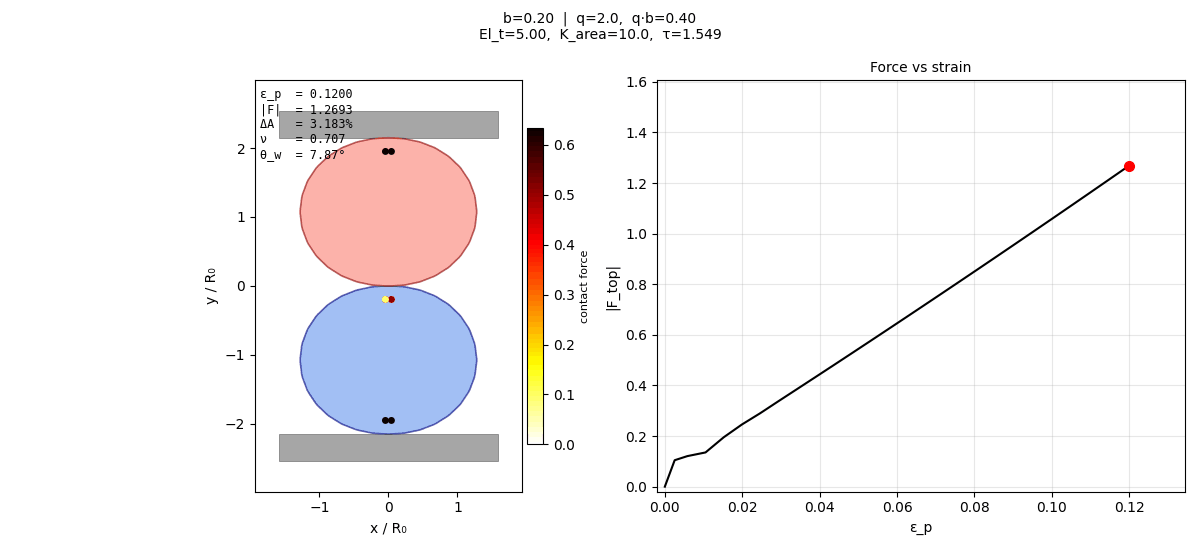
\includegraphics[width=\linewidth]{figures/S4_frame.png}
  \caption{%
    \textbf{Movie~S4} (\texttt{movies/S4\_q2p0\_intermediate.gif}):
    Single squeeze at $q = 2.0$ ($q \cdot b = 0.40$, $\numes \approx 0.69$,
    $\dA \approx 2.1\%$).  The disk conserves area moderately well;
    significant lateral bulging is visible.  This regime is intermediate
    between area-compressible and shape-deformable.
    Still shown: maximum compression.
  }
  \label{fig:S4}
\end{figure}

%%------------------------------------------------------------------
\section*{Movie S5 — Shape-deformable disk ($q = 10$, $\numes \approx 0.88$)}
%%------------------------------------------------------------------

\begin{figure}[htb]
  \centering
  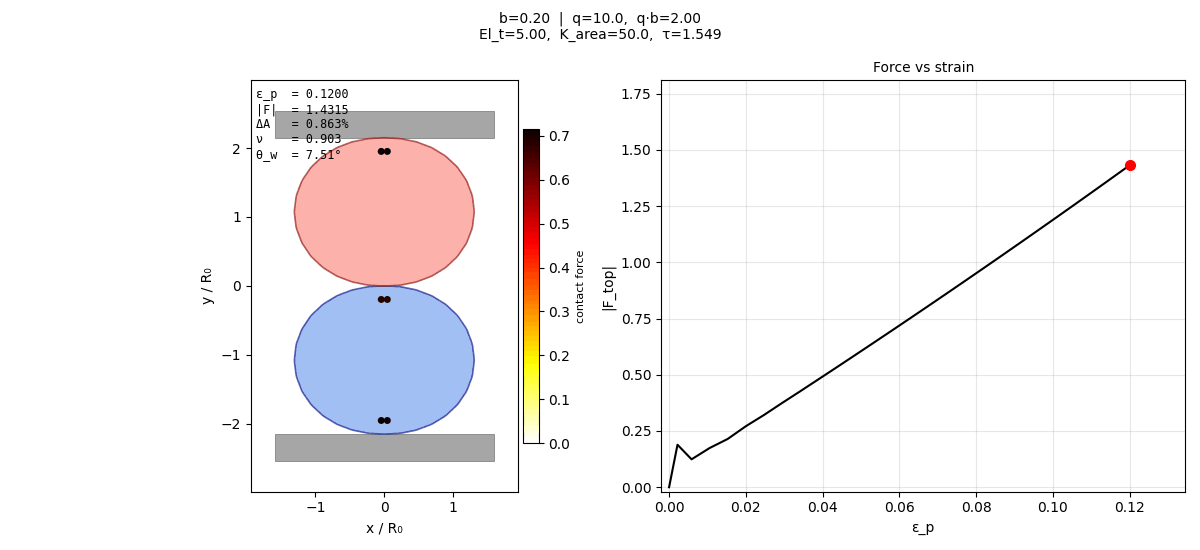
\includegraphics[width=\linewidth]{figures/S5_frame.png}
  \caption{%
    \textbf{Movie~S5} (\texttt{movies/S5\_q10p0\_shape\_deformable.gif}):
    Single squeeze at $q = 10$ ($q \cdot b = 2.0$, $\numes \approx 0.88$,
    $\dA \approx 0.57\%$).  The area is well conserved; the deformation is
    almost purely shape change.  The disk develops a pronounced ``peanut''
    profile under strong compression, with wide flat contact zones and
    equatorial bulge.  Still shown: maximum compression.
  }
  \label{fig:S5}
\end{figure}

%%------------------------------------------------------------------
\section*{Movie S6 — Nearly incompressible disk ($q = 50$, $\numes \approx 0.94$)}
%%------------------------------------------------------------------

\begin{figure}[htb]
  \centering
  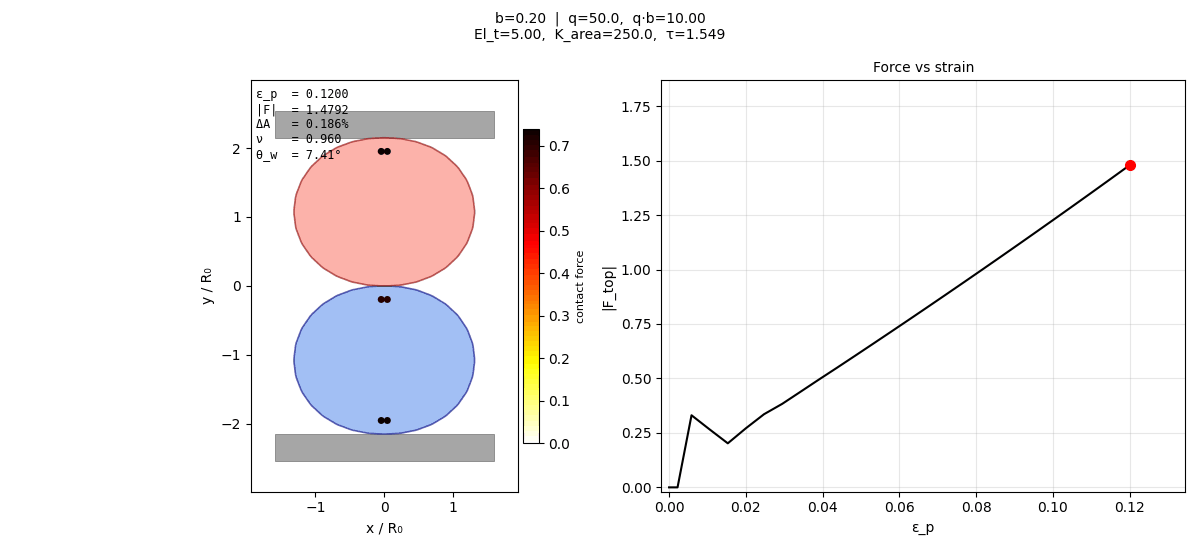
\includegraphics[width=\linewidth]{figures/S6_frame.png}
  \caption{%
    \textbf{Movie~S6} (\texttt{movies/S6\_q50p0\_nearly\_incompressible.gif}):
    Single squeeze at $q = 50$ ($q \cdot b = 10.0$, $\numes \approx 0.94$,
    $\dA \approx 0.12\%$).  Near the incompressible limit; the disk conserves
    area to within $0.1\%$ and deforms entirely by shape change.  The lateral
    bulge is maximal; the contact zone spans a large fraction of the perimeter.
    This is the ``rubber-like'' or ``jello-like'' end of the squishiness axis.
    Still shown: maximum compression.
  }
  \label{fig:S6}
\end{figure}

%%------------------------------------------------------------------
\section*{Movies S7a--S7c — Three-body collisions: momentum conservation}
%%------------------------------------------------------------------

Movies~S7a--S7c show three-body disk collision events using \texttt{step\_rb()}.
Two identical EPD disks approach a stationary target from opposite angles;
per-frame $\Delta p_x/p_0$ and $\Delta p_y/p_0$ are overlaid as text.
Three configurations are shown: elastic ($\alpha_d = 0$, $q = 1$),
damped ($\alpha_d = 2$, $q = 1$), and rubber-like ($\alpha_d = 0$, $q = 10$).
Total linear momentum is conserved to $|\Delta p|/p_0 < 2 \times 10^{-15}$ and
angular momentum to $|\Delta L|/L_0 < 1.4 \times 10^{-14}$ in all cases.
See \texttt{src/validation/rb\_extension\_benchmarks.py}.

\begin{figure}[htb]
  \centering
  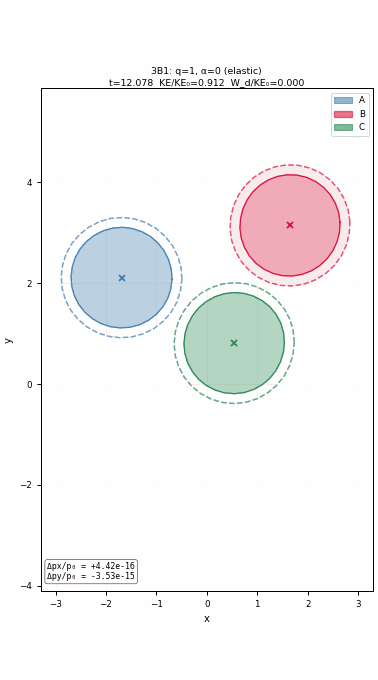
\includegraphics[width=0.85\linewidth]{figures/S7a_frame.png}\\[4pt]
  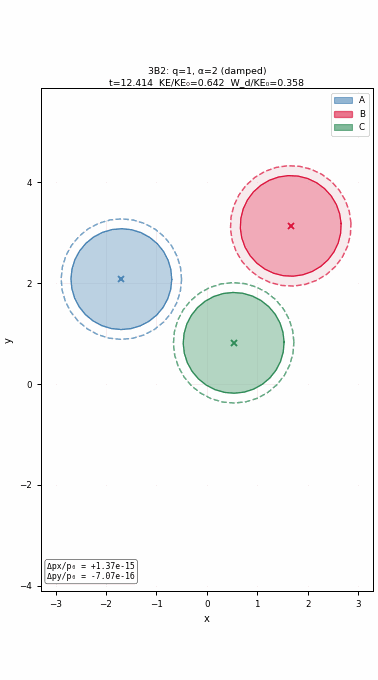
\includegraphics[width=0.85\linewidth]{figures/S7b_frame.png}\\[4pt]
  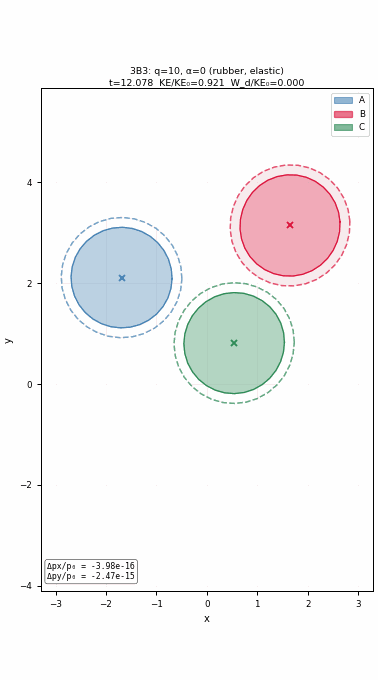
\includegraphics[width=0.85\linewidth]{figures/S7c_frame.png}
  \caption{%
    \textbf{Movies~S7a--S7c}
    (\texttt{movies/extension\_3B\{1,2,3\}.gif}):
    Three-body collisions at elastic ($\alpha_d = 0$, $q = 1$, top),
    damped ($\alpha_d = 2$, $q = 1$, middle), and
    rubber-like ($\alpha_d = 0$, $q = 10$, bottom) conditions.
    Per-frame momentum residuals are displayed; all remain at machine
    precision throughout.  Stills shown at mid-collision.
  }
  \label{fig:S7}
\end{figure}

%%------------------------------------------------------------------
\section*{Movies S8a--S8d — EllipseParticle: shape generalization}
%%------------------------------------------------------------------

Movies~S8a--S8d show free-flight collisions of \texttt{EllipseParticle}
objects (semi-axes $a = 1.5$, $b = 0.8$, $N = 32$ equal-arc-length nodes).
Four configurations are covered: E1 (equal ellipses, head-on, no spin),
E2 (equal ellipses, oblique impact with initial spin $\omega_0 = \pm 0.8$),
E3 (different-size oblique collision with spin), and
E4 (same moment of inertia, different mass/density, with spin).
Angular momentum is conserved to $|\Delta L|/L_0 \leq 8 \times 10^{-13}$
in all four cases.
See \texttt{src/validation/ellipse\_collision\_benchmark.py}.

\begin{figure}[htb]
  \centering
  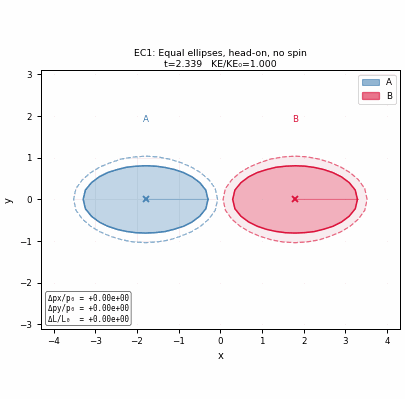
\includegraphics[width=0.85\linewidth]{figures/S8a_frame.png}\\[4pt]
  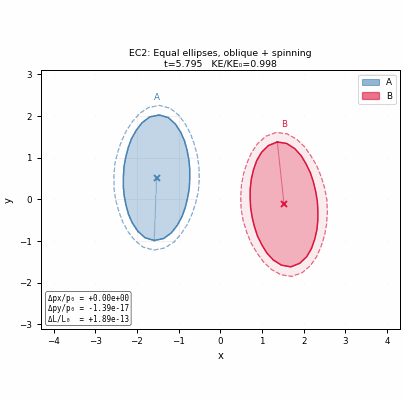
\includegraphics[width=0.85\linewidth]{figures/S8b_frame.png}\\[4pt]
  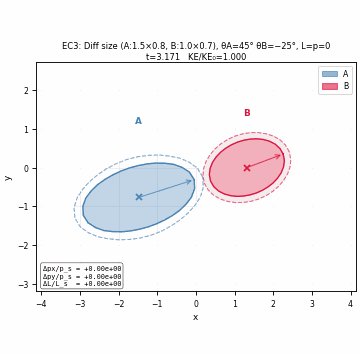
\includegraphics[width=0.85\linewidth]{figures/S8c_frame.png}\\[4pt]
  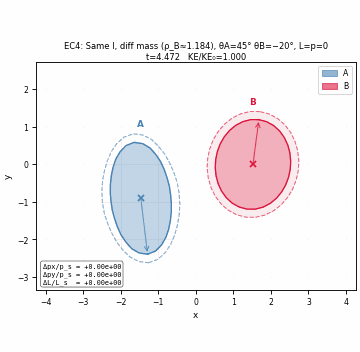
\includegraphics[width=0.85\linewidth]{figures/S8d_frame.png}
  \caption{%
    \textbf{Movies~S8a--S8d}
    (\texttt{movies/ellipse\_EC\{1,2,3,4\}.gif}):
    EllipseParticle collision configurations E1--E4 (top to bottom).
    The rigid-body decomposition conserves angular momentum to machine
    precision regardless of particle shape, mass asymmetry, or initial spin.
    Stills shown at mid-collision.
  }
  \label{fig:S8}
\end{figure}

%%------------------------------------------------------------------
\section*{Movie S9 — Emulsion capillary-wave ringdown}
%%------------------------------------------------------------------

Movie~S9 shows a single emulsion droplet ($N = 120$, $K_\mathrm{area} = 50$,
$\kappa = 0.02$, $\alpha = 5.0$) released from a 10\% elliptical deformation and
allowed to relax.  The $n = 2$ capillary-wave mode rings down over $\approx 3$
oscillation periods; the exponential amplitude decay gives the measured damping
rate $\alpha_\mathrm{meas} \approx 2.50\,\tau_0^{-1}$, consistent with the
near-critical damping target $\alpha_\mathrm{crit} = 2\omega_2 \approx 5.46\,\tau_0^{-1}$.
See \texttt{src/validation/emulsion\_paper\_figures.py}, Benchmark~C.

%%------------------------------------------------------------------
\section*{Movie S10 — Emulsion T1 topological rearrangement}
%%------------------------------------------------------------------

Movie~S10 shows the T1-event benchmark: a center droplet squeezed vertically
between two pinned neighbor droplets and two horizontal walls ($d = 1.5\,R_0$
gap, $N = 120$, $K_\mathrm{area} = 50$).  The center droplet elongates
vertically, passes through the gap, and snaps horizontally to rest between
the two neighbors --- the elementary topological rearrangement of an emulsion.
Area change during passage is $\Delta A < 2\%$; lateral symmetry is maintained
to within $< 1\%$ of $R_0$ throughout.
See \texttt{src/validation/emulsion\_paper\_figures.py}, Benchmark~D.

%%------------------------------------------------------------------
\section*{Movie S11 — Emulsion droplet falling under gravity ($\mathrm{Bo} = 0.10$)}
%%------------------------------------------------------------------

Movie~S11 shows a single droplet falling freely under gravity at
$\mathrm{Bo} = 0.10$ ($N = 120$, $K_\mathrm{area} = 50$).  The droplet
accelerates from rest, reaches terminal-like behavior, and develops a
visible oblate deformation: the leading (bottom) edge flattens while the
trailing (top) edge rounds, giving a sag ratio
$(R_\mathrm{top} - R_\mathrm{bot})/R_0 \approx 0.065$.  Trajectory error
relative to ballistic free-fall is $< 3 \times 10^{-4}$ in units of $R_0$.
See \texttt{src/validation/emulsion\_paper\_figures.py}, Benchmark~E.

%%------------------------------------------------------------------
\section*{Movie S12 — Terminal velocity with Stokes drag ($\mathrm{Oh} = 0.25$, $g = 0.05$)}
%%------------------------------------------------------------------

Movie~S12 shows a single emulsion droplet ($N = 36$, $\kappa = 0.02$,
$\mathrm{Oh} = 0.25$, $g = 0.05$) released from rest near the top of a tall box
($L_x = 20$, $L_y = 60$) and falling under gravity with Stokes drag.
The right panel shows a real-time speed gauge comparing the measured $|v_{{\rm cm},y}|$
to the theoretical terminal velocity $v_t = g/(2\,\mathrm{Oh}) = 0.10$.
The droplet reaches $v_t$ within the first third of the trajectory; subsequent
evolution confirms steady terminal-velocity descent.
See \texttt{papers/summary\_of\_methods/scripts/test\_E\_movies.py}, Benchmark~E1.

%%------------------------------------------------------------------
\section*{Movie S13 — Shear flow: drift and rotation ($\Gamma = 0.05$, $\mathrm{Oh} = 0.5$)}
%%------------------------------------------------------------------

Movie~S13 shows a single emulsion droplet ($N = 36$, $\kappa = 0.02$,
$\mathrm{Oh} = 0.5$) in a simple shear background flow $U_x = \Gamma y$,
$U_y = 0$ ($\Gamma = 0.05$).  The droplet drifts to the right at rate
$\dot{x}_{\rm cm} = \Gamma y_{\rm cm}$ while rotating clockwise at the predicted
Jeffery rate $\omega = -\Gamma/2 = -0.025$.  Background shear arrows indicate
the local flow direction and magnitude; the right panel shows the instantaneous
rotation rate $\omega(t)$ relative to the theoretical value $\omega_{\rm theory}$.
See \texttt{papers/summary\_of\_methods/scripts/test\_E\_movies.py}, Benchmark~E3.

\end{document}
